% Configuración del tipo páginas
        \documentclass[12pt, a4paper,english,spanish]{amsart}
        \parindent = 10 pt
        \parskip=1.5pt 
        \usepackage[width=15.5cm, left=3cm, top=2.5cm, height= 24.5cm]{geometry}

% Paquete para reconocer la separación en sílabas en español
        \usepackage[utf8]{inputenc}
        \usepackage[spanish]{babel}

% Paquetes especiales
        \usepackage{amsmath}
        \usepackage{amsfonts}
        \usepackage{amssymb}
        \usepackage{upgreek}
        \usepackage{ifthen}
        \usepackage{alltt}
        \usepackage[pdftex]{graphicx}
        \usepackage{subfig}
        \usepackage{float}
        \usepackage{mathtools}
        \usepackage{amsthm}
        \usepackage[vlined,tworuled,commentsnumbered,linesnumbered]{algorithm2e}
        \usepackage{hyperref} %links
        \usepackage{etoolbox} %set verbatim spacing


        
\begin{document}
%setting verbatim spacing
\makeatletter
\preto{\@verbatim}{\topsep=0pt \partopsep=0pt }
\makeatother

\begin{center}
~\\
~\\
~\\
~\\
~\\
~\\
~\\
~\\
~\\
~\\
~\\
~\\
   \Large\textbf{Trabajo práctico de fin de cursada}\\
   \Large\textbf{Sistemas complejos en maquinas paralelas}\\
   \large\textit{Alejandro Martín Ventura}\\
\end{center}
\newpage

\begin{section}{Introducción}
Los flujos son gobernados por ecuaciones diferenciales parciales, que representan las leyes de conservación de masa, momento y energía. La dinámica de fluidos computacional se encarga de resolver esas ecuaciones diferenciales utilizando técnicas de análisis numérico. Las computadoras son utilizadas para realizar los cálculos requeridos para simular la interacción entre líquidos, gases y superficies definidas por las condiciones de borde. Disponer de mas poder computacional es útil para disminuir el tiempo requerido para realizar las simulaciones, o aumentar la calidad de los resultados.

Para poder aumentar el poder computacional disponible, se utilizan a menudo, técnicas de computación en paralelo. La computación en paralelo consiste en la realización de varios cálculos, o la ejecución de varios procesos de forma simultanea. Para poder aprovechar esta forma de calculo, los problemas grandes deben ser divididos en problemas mas pequeños que puedan resolverse independientemente, o con el intercambio de solo pequeñas cantidades de información entre los agentes que resuelven cada parte.

Para facilitar el trabajo de la programación de una solución paralela, se utilizara en este trabajo MPI (message passing interface). MPI es un sistema de pasaje de parámetros estandarizado y portable, que puede ser utilizado en una gran variedad de arquitecturas paralelas, y tiene un uso muy difundido en el campo de la computación de alto rendimiento. 

En este trabajo se realizara una simulación de las ecuaciones de Navier Stokes bidimensionales. Concretamente se resolverá el problema del flujo interno en un contenedor rectangular, en cuyo centro se encuentra situada una hélice que perturba el fluido creando así un campo de velocidades. Esta simulación es de particular interés para aquellos que trabajen con dispositivos similares, sean estos reactores químicos, enfriadores, o torres de mezclado. 

\end{section}



\newpage

\begin{section}{Modelo}
Las ecuaciones de Navier Stokes son ecuaciones diferenciales en derivadas parciales, no lineales e inhomogéneas. Ademas son parabólicas, ya que tienen un termino difusivo distinto de cero.

En nuestro caso trabajaremos con las ecuaciones para fluidos incompresibles.
\begin{center}
$\nabla \cdot v_e = 0$\\
$\frac{\partial v_e}{\partial t} + (v_e \cdot \nabla)v_e = -\frac{1}{\rho}\nabla p+\nu \nabla^2v_e$
\end{center}

Donde p es la presión, v la velocidad, $\rho$ la densidad, y $\nu$ la viscosidad. La primera ecuación define la conservación de la masa para densidad constante $\rho$. 
Los valores que se utilizaran para cada una de estas constantes son 0.01 para la viscocidad, 1 para la densidad, ya que son consistentes con los valores para el agua en unidades del sistema internacional.
Para acoplar la velocidad y la presión debemos realizar dos pasos. Primero aplicamos divergencia a ambos miembros de la segunda ecuación aplicando luego la primera ecuación sobre el resultado. Se obtiene el siguiente sistema de ecuaciones, donde la primera ecuación representa la velocidad en la dirección de u, y la segunda la velocidad en la dirección de v. Es decir, $v=(u,v)$. Ademas agregamos a estas ecuaciónes, los terminos $F_u$ y $F_v$, por ahora genericos, que corresponderan a la fuerza ejercida por la helice en las componentes u y v.
~\\

\begin{center}

$\frac{\partial u}{\partial t} + u \frac{\partial u}{\partial x} + v \frac{\partial u}{\partial y} = -\frac{1}{\rho} \frac{\partial p}{\partial x} + \nu ( \frac{\partial ^2 u}{\partial x^2} + \frac{\partial ^2 u}{\partial y^2}) + F_u$
~\\
$\frac{\partial v}{\partial t} + u \frac{\partial v}{\partial x} + v \frac{\partial v}{\partial y} = -\frac{1}{\rho} \frac{\partial p}{\partial y} + \nu ( \frac{\partial ^2 v}{\partial x^2} + \frac{\partial ^2 v}{\partial y^2}) + F_v$
~\\
$\frac{\partial ^2 p}{\partial x^2} + \frac{\partial ^2 p}{\partial y^2} = - \rho(\frac{\partial u}{\partial x} \frac{\partial u}{\partial x}  + 2 \frac{\partial u}{\partial y}  \frac{\partial v}{\partial x} + \frac{\partial v}{\partial y} \frac{\partial v}{\partial y}  )$


\end{center}

Las ecuaciones están ahora parcialmente acopladas, pasaremos ahora a discretizarlas.
\end{section}




\begin{section}{Discretización}
Comenzaremos con algunas definiciones. al modelar con diferencias finitas, se utilizan ciertos reemplazos de los operadores diferenciales conocidos como discretizaciones. Como su nombre indica, estos son versiones discretas de los operadores, y se los usa bajo el supuesto de que en el limite se comportan de forma similar. Pasaremos ahora a definir algunas discretizaciones que serán utilizadas en al hacer el pasaje.
~\\
~\\
\begin{minipage}{\linewidth}

Centradas de primer orden:
\begin{center}

~\\
$\frac{dU}{dx} = \frac{U^{n}_{i+1,j} - U^{n}_{i-1,j}}{2dx} $
~\\
~\\
$\frac{dU}{dy} = \frac{U^{n}_{i,j+1} - U^{n}_{i,j-1}}{2dy} $
~\\
~\\
$\frac{dU}{dt} = \frac{U^{n+1}_{i,j} - U^{n-1}_{i,j}}{2dt} $
~\\
\end{center}

\end{minipage}
\begin{minipage}{\linewidth}



Centradas de segundo orden:
\begin{center}

~\\
$\frac{d^{2}U}{dx^{2}} = \frac{ U^{n}_{i+1,j} - 2*U^{n}_{i,j} + U^{n}_{i-1,j}}{dx^2}$
~\\
~\\
$\frac{d^{2}U}{dy^{2}} = \frac{ U^{n}_{i,j+1} - 2*U^{n}_{i,j} + U^{n}_{i,j-1}}{dx^2}$
~\\
~\\
$\frac{d^{2}U}{dt^{2}} = \frac{ U^{n+1}_{i,j} - 2*U^{n}_{i,j} + U^{n-1}_{i,j}}{dt^2}$
~\\
\end{center}

\end{minipage}
\begin{minipage}{\linewidth}

Adelantadas de primer orden:
\begin{center}

~\\
$\frac{dU}{dx} = \frac{U^{n}_{i+1,j} - U^{n}_{i,j}}{dx} $
~\\
~\\
$\frac{dU}{dy} = \frac{U^{n}_{i,j+1} - U^{n}_{i,j}}{dy} $
~\\
~\\
$\frac{dU}{dt} = \frac{U^{n+1}_{i,j} - U^{n}_{i,j}}{dx} $
~\\
\end{center}

\end{minipage}
\begin{minipage}{\linewidth}


Atrasadas de primer orden:
\begin{center}

~\\
$\frac{dU}{dx} = \frac{U^{n}_{i,j} - U^{n}_{i-1,j}}{dx} $
~\\
~\\
$\frac{dU}{dy} = \frac{U^{n}_{i,j} - U^{n}_{i,j-1}}{dy} $
~\\
~\\
$\frac{dU}{dt} = \frac{U^{n}_{i,j} - U^{n-1}_{i,j}}{dx} $
~\\
\end{center}
\end{minipage}
~\\

\begin{minipage}{\linewidth}

Reemplazando estas discretizaciones en las ecuaciones semi-acopladas de Navier Stokes y obtenemos: 
\begin{center}
~\\

~\\
$\frac{u_{i,j}^{n+1}-u_{i,j}^{n}}{\Delta t}+u_{i,j}^{n}\frac{u_{i,j}^{n}-u_{i-1,j}^{n}}{\Delta x}+v_{i,j}^{n}\frac{u_{i,j}^{n}-u_{i,j-1}^{n}}{\Delta y}
=-\frac{1}{\rho}\frac{p_{i+1,j}^{n}-p_{i-1,j}^{n}}{2\Delta x}+\nu (\frac{u_{i+1,j}^{n}-2u_{i,j}^{n}+u_{i-1,j}^{n}}{\Delta x^2}+\frac{u_{i,j+1}^{n}-2u_{i,j}^{n}+u_{i,j-1}^{n}}{\Delta y^2}) + Fu$
~\\
~\\
~\\

$\frac{v_{i,j}^{n+1}-v_{i,j}^{n}}{\Delta t}+u_{i,j}^{n}\frac{v_{i,j}^{n}-v_{i-1,j}^{n}}{\Delta x}+v_{i,j}^{n}\frac{v_{i,j}^{n}-v_{i,j-1}^{n}}{\Delta y}=-\frac{1}{\rho}\frac{p_{i,j+1}^{n}-p_{i,j-1}^{n}}{2\Delta y}
+\nu(\frac{v_{i+1,j}^{n}-2v_{i,j}^{n}+v_{i-1,j}^{n}}{\Delta x^2}+\frac{v_{i,j+1}^{n}-2v_{i,j}^{n}+v_{i,j-1}^{n}}{\Delta y^2}) + Fv$
~\\
~\\
~\\

$\frac{p_{i+1,j}^{n}-2p_{i,j}^{n}+p_{i-1,j}^{n}}{\Delta x^2}+\frac{p_{i,j+1}^{n}-2*p_{i,j}^{n}+p_{i,j-1}^{n}}{\Delta y^2} 
=\rho[\frac{1}{\Delta t}(\frac{u_{i+1,j}-u_{i-1,j}}{2\Delta x}+\frac{v_{i,j+1}-v_{i,j-1}}{2\Delta y})$
\end{center}

\end{minipage}
~\\
~\\

\begin{minipage}{\linewidth}
Aquí en la ultima ecuación podemos ver que no se reemplazó directamente cada operador mediante las ecuaciones de discretización, sino que se agregó un termino temporal, sin que hubiera en principio información sobre el tiempo en la ecuación de la presión. Este cambio se hace con el objetivo de terminar de acoplar la ecuación de la presión con las ecuaciones de velocidad. La derivación de esta solución no se presentará en este trabajo.
~\\

Cabe aclarar que al discretizar, se puede modelar el sistema mediante un método implícito o explicito. Un método implícito, o parcialmente implícito, incluiría una ponderación entre los valores de las variables en la iteración n, y la iteración n+1. En este trabajo utilizaremos un método explicito, ya que el sistema de ecuaciones determinado por un método explicito es lineal, y resulta en relaciones donde un elemento en la iteración n+1 depende de otros en la iteración n, pudiendo entonces realizarse los reemplazos en las matrices que representan el sistema de forma directa, y resultando así en una implementación mas sencilla. Un método implícito da como resultado un sistema no lineal, en el cual hay que hacer uso de algún método de resolución de sistemas no lineales, como punto fijo, lo cual aumenta la complejidad de la implementación.

\end{minipage}
\end{section}


\begin{section}{Condiciones de contorno}
El sistema fisico esta compuesto por un recipiente rectangular que contiene un liquido dentro. Ademas una helice en el centro, cuyas aspas son rectas y de exactamente la misma longitud a distintas alturas, perturba el liquido produciendo en el cambios de velocidad. 
Para la simulación se aprovechara la simetria del problema para modelarlo en dos dimensiones. Se tomara entonces un corte horizontal del reactor. El sistema, como sera modelado, consiste entonces de un plano horizontal, cuyos vértices y aristas representan las paredes del recipiente, un espacio dentro que representa el fluido, y segmentos en el centro que representan la posición de las aspas de la helice. Definir la cantidad de aspas en la helice es sencillo, basta con cambiar las condiciónes en un condicional que logra que se trate distinto a los elementos de dluido donde deberia estar un aspa. En el presente trabajo se realizó la experimentación con una unica aspa ya que esto aporta mayor claridad a la hora de evaluar el comportamiento del fluido.
~\\
~\\
Las condiciones de contorno para Las ecuaciones de velocidad no presentan mayores complejidades, se establece la velocidad del fluido en los bordes del contenedor como cero en ambas direcciones, u y v. Estas velocidades no se cambian en las subsecuentes iteraciones del programa ya que representan las paredes del contenedor que se mantienen quietas en todo momento en el sistema físico real.
En cuanto a la ecuación de la presión, utilizar una presión de cero en el contorno no seria realista dado que la presencia de una  presión muy baja produce la atracción del fluido circundante. Una forma de deducir el valor correcto de la presión en los bordes del contenedor es utilizar las ecuaciones de Newton. Si un elemento de fluido realiza una fuerza en la pared del contenedor, dado que esta no se mueve, devuelve una fuerza igual al elemento de fluido. Realizando este calculo, se llega a una condición de igualdad entre el elemento de borde y el elemento de fluido que se encuentre junto a este. Básicamente lo que ese resultado nos dice es que el valor de presión para un elemento de borde debe ser el mismo que el del elemento de fluido que esta junto a el, pudiendo entonces solucionar este aspecto de la simulación simplemente copiando el valor del elemento de fluido mas cercano a cada elemento de borde en cada iteración.\\
Finalmente para las condiciones iniciales, se estableció la velocidad en u y en v en cero para todo el sistema.

\end{section}

\newpage

~\\
~\\

\begin{section}{Implementacion}
La implementación fue realizada casi completamente en C++, excepto por el graficador que se escribió en Matlab. 
~\\
~\\
Corriendo de forma no paralela, el programa define las matrices U2, U2, V1, V2, P1, P2, que representan el estado del sistema en una iteración para la velocidad en u, en v, y la presión, y luego estas mismas en la iteración siguiente. 
~\\
~\\
Se definen las condiciones iniciales del problema, y luego se utiliza el metodo explicito explicado anteriormente para calcular los nuevos valores del sistema. Estos son guardados en U2, V2, y P2. Seguido de esto el programa reemplaza los valores de U1, V1, y P1, por aquellos de U2, V2 y P2, quedado así preparado para la siguiente iteración. 
~\\
~\\
Una salvedad es que al realizar el calculo de los nuevos valores, si un elemento forma un angulo respecto del centro del sistema que es congruente con aquel que debería tener el aspa para el tiempo de esa iteración, entonces a ese elemento se le aplica una fuerza de la forma $F = A \delta v^2$, donde A es el área compartida por los elementos, y $\delta v$ es la diferencia de velocidad, para ese punto, entre el aspa y el fluido. Esta diferencia es calculada restando componente a componente, los elementos correspondientes de las matrices U1 y V1, y la velocidad tangencial del aspa en ese punto, que resulta de multiplicar la velocidad angular por el radio elemento menos el punto central del sistema. 
~\\
~\\
Se implementó también una clase mat2, que representa una matriz, y que contiene un puntero a un arreglo de números de punto flotante de doble precisión y dos enteros que representan el tamaño en filas y columnas de la matriz. Ademas la clase cuenta con funciones que realizan la abstracción de indexar en el arreglo calculando la posición del elemento buscado como la columna pedida, mas la fila pedida multiplicada por la cantidad de columnas. Esta clase también cuenta con una función de impresión que escribe los elementos de la matriz en formato separado por espacios.
~\\
~\\
En cuanto a la paralelización, como se comentó anteriormente se utilizó MPI. El procedimiento básico es el siguiente.
\begin{itemize}

\item Se inicializan el comunicador, cantidad de procesos y demás variables pertinentes a MPI.
\item Se calcula una división del espacio de trabajo por filas, para saber de que sección sera responsable cada proceso.
\item El proceso cero define las matrices del sistema y sus condiciones iniciales y luego envía la sección horizontal correspondiente de la matriz a cada proceso. Luego calcula la sección que le corresponde a el mismo.
\item Los otros procesos reciben las secciones que les corresponden.
\item Todos los procesos ejecutan una función encargada de procesar la simulación.
\item Dentro de esta función, se encuentra un ciclo en el cual realizan los cálculos pertinentes a la simulación, y al terminar una iteración, cada proceso envía los nuevos valores de los elementos que pertenecen a su sección, pero que son necesarios para que procesos vecinos calculen la siguiente iteración de sus elementos.
\item Cada proceso recibe los valores enviados por los procesos vecinos.
\item Cada proceso chequea el numero de iteración, y en caso de que sea multiplo de cierto valor prefijado, envía su sección entera al proceso cero para que este imprima. Luego el proceso cero reúne todas las secciones armando las matrices completas.
\item Si es el caso, el proceso cero imprime las matrices U y V por la salida estándar.
\item Luego de esto el ciclo descripto en el paso seis termina, y se vuelve a ejecutar. En caso de haber llegado al tiempo máximo de la simulación, todos los procesos retornan de la función, y luego de la función principal.
~\\
~\\

Aquí cabe aclarar algunas cosas. Primero, la impresión realizada por el proceso cero, imprime U y V de un tiempo, y U yV del tiempo siguiente de forma contigua. Es la rutina de Matlab la que se encarga de separar y conferir significado a esos datos. 
~\\
Por otro lado, como se dijo el trabajo se divide entre los procesos otorgando a cada uno una franja horizontal del sistema, es decir, se le otorga un numero de fila inicial, y un numero de fila final que determinan los rangos en los que el proceso trabajará. Esta división no es optima, ya que otras formas de dividir el trabajo resultan en un menor intercambio de información entre los procesos durante la simulación, que es un factor importante a la hora de optimizar la velocidad de ejecución del programa. La decisión de utilizar una división horizontal es simplemente por simplicidad del código.
~\\
~\\
Otro detalle es que si bien se dice que cada proceso toma los valores que le faltan para la iteración siguiente, de los procesos vecinos, en cada iteración. En el caso del proceso cero, o del ultimo, solo interactúan con un proceso vecino, ya que las condiciones de contorno no se modifican, o son calculadas por ellos mismos ya que no dependen de elementos extra.
~\\
~\\ Ademas, durante la simulación no se crean ni se destruyen matrices, sino que estas son reutilizadas cambiando los valores que contienen para no perder tiempo manejando memoria.
~\\
~\\
Por ultimo se hablará sobre los valores de la malla, es decir, la división del sistema físico representada por las matrices. Durante el testeo del programa se encontró que la solución a veces puede ser inestable. En particular cuando los valores de dx y dy son muy chicos, o el valor de dt es grande, la simulación se vuelve inestable, acumulando error numérico y desbordando la precisión máxima de los tipos numéricos de C++. 
~\\
~\\
Llegado a este punto el programa emite un mensaje de error, avisando que recibió durante la simulación NaN como resultado de un calculo. Sucedido esto el programa termina, y es responsabilidad del usuario del mismo, aumentando el valor del tamaño de los elementos, haciendo menos fina la malla espacialmente, o disminuyendo el tamaño del salto temporal entre iteraciones, haciendo mas fina la simulación en el tiempo. Cualquiera de estas dos medidas, elegido el valor correcto, resuelve el problema de la estabilidad. 
~\\
~\\
Se aclara también que a veces una simulación se vuelve inestable, pero termina antes de que los valores calculados desborden de la precisión numérica de las variables, en ese caso la simulación sera incorrecta, incluso no habiendo mensaje de error alguno. 
~\\
~\\
Sin embargo, algo bueno de las simulaciones de dinámica de fluidos por diferencias finitas, es que muy a menudo, cuando se vuelven inestables, lo hacen de una forma muy clara, que no se comporta para nada como un fluido, se recomienda entonces hecha un vistazo, siempre que se pueda, a algún gráfico de los resultados de la simulación para comprobar que esta se mantuvo estable.
\end{itemize}

\end{section}



\newpage

\begin{section}{Experimentación}
 No se realizaron estudios in vitro, comparando la simulación contra un fluido real bajo las mismas condiciones. Se realizaron dos videos uno es un \href{https://www.youtube.com/watch?v=D8JOELu8uAs}{mapa de velocidad total codificado por color}, donde el color codifica la velocidad y el otro un \href{https://www.youtube.com/watch?v=_JisfmOIEdU}{campo vectorial}
 campo vectorial donde cada flecha representa la velocidad y dirección del fluido en cada punto. La simulación parece reflejar el comportamiento esperado por un fluido. No se realizaron mas estudios cualitativos.
~\\
~\\
Fueron realizados estudios de rendimiento, tratando de medir el impacto de la ejecución en paralelo. Como marco teórico de esta sección, se utilizó por un lado la Ley de Amdahl, midiendo así el speedup  $S(n,p) = \frac{T_{ser}(n) }{ T_{par}(n,p)}$  a trabajo fijo aumentando la cantidad de procesadores, y por otro la Ley de Gustavson para la cual medimos el trabajo realizado por cantidades cada vez mas grandes de recursos de procesamiento a tiempo constante, y luego calculamos la eficiencia $E(n,p) = \frac{S(n,p)}{p}$. Donde $ T_{ser}(n)$  es el tiempo que tarda el programa en su versión serial para una entrada de tamaño n, y $T_{par}(n,p)$  es el tiempo que tarda el programa paralelo para una entrada de tamaño n y cantidad de procesos p.

\begin{subsection}{Ley de Amdahl}
~\\
La Ley de Amdahl nos da el speedup teórico en la ejecución de una tarea que consta de una cantidad de trabajo fijo al incrementar los recursos del sistema.
~\\
~\\
Llevada al limite, sirve para calcular la mejora máxima posible para una tarea que consta de una parte paralelizable, y una parte serial que no puede ser efectivamente paralelizada.
~\\
La formulación matemática de la Ley de Amdahl es la siguiente:
~\\
~\\
\begin{center}
$S(s) \leq  \frac{1}{(1-p)+\frac{p}{s}}$
\end{center}
~\\
~\\
Donde S es el speedup total, s el speedup de la parte del programa que se favorece por el paralelismo, y p es la proporción de tiempo que era ocupada por la parte del programa que tiene speedup alguno. Se asume que todo el tiempo que no corresponde a p, o sea 1-p, se mantiene igual. Un resultado directo de esta ley es que incluso utilizando infinitos recursos, no puede aumentarse el speedup mas que:

~\\
~\\
\begin{center}
$S(s) \leq  \frac{1}{1-p}$
\end{center}
~\\
~\\
\newpage
Para este experimento se quiere dejar fija la cantidad de trabajo total realizado, y medir como cambia la velocidad al agregar unidades de procesamiento. 
~\\
~\\
El programa fue ejecutado en una red ethernet con 21 maquinas, cada una disponiendo de 4 núcleos. Al momento de realizar la experimentación, estas maquinas estaban siendo utilizadas, a razón de dos nucleos por maquina, con lo cual se disponía de 42 núcleos para procesar la prueba. Los resultados son los siguientes:
~\\
\begin{verbatim}
nucleos time
30      43.681s
25      45.017s
20      49.776s
15      56.197s
12      69.997s
10      82.439s
9       94.491s
8       102.819s
6       142.737s
5       171.753s
3       343.118s
1       867.247s
\end{verbatim}
~\\
Con lo cual los speedups serían:
~\\
\begin{verbatim}
nucleos speedup

30      19.8541013255
25      19.2648777129
20      17.4229950177
15      15.4322650675
12      12.3897738475
10      10.5198631716
9       9.1780910351
8       8.434695922
6       6.0758387804
5       5.0493848725
3       2.5275473744
1       1

\end{verbatim}

En el siguiente gráfico se pueden ver los datos de la tabla.
~\\
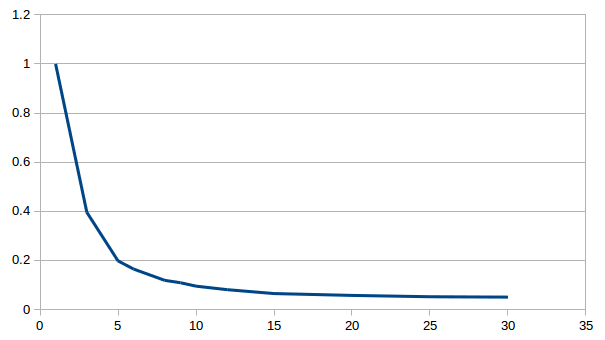
\includegraphics{AmdahlSpeedup}

Como puede apreciarse, el speedup tiende a disminuir al aumentar mucho la cantidad de nucleos, perdiendo approximadamente un tercio del rendimiento al alcanzar los 30.
\end{subsection}


\begin{subsection}{Ley de Gustavson}
~\\
La Ley de Gustafson calcula el speedup teórico para una tarea de tiempo de ejecución fijo al incrementar los recursos de un sistema. Al aplicar la Ley de Gustavson, lo que varia no es el tiempo de ejecución, sino la cantidad de trabajo realizado. 
~\\
La formulación matemática de la Ley de Gustavson es la siguiente:
~\\
~\\
\begin{center}
$S(s) = p - \alpha(p-1)$
\end{center}
~\\
~\\
Donde S es el speedup, p es el número de procesadores, y $\alpha$ la parte no paralelizable del proceso. Notar que si se aumenta notablemente la el trabajo total en la sección paralelizable, haciendo que la proporción de trabajo serial $\alpha$ sea muy pequeña, esto resulta en algo muy similar a $S(s) = p$
\newpage
Con los datos obtenidos anteriormente, se obtienen los siguientes datos de eficiencia:
\begin{verbatim}
nucleos     eficiencia

30			0.6618033775
25			0.7705951085
20			0.8711497509
15			1.0288176712
12			1.032481154
10			1.0519863172
9			1.0197878928
8			1.0543369902
6			1.0126397967
5			1.0098769745
3			0.8425157915
1			1
\end{verbatim}

En el siguiente grafico se puede observar la perdida de linealidad de estas mediciones al crecer la cantidad de procesadores:

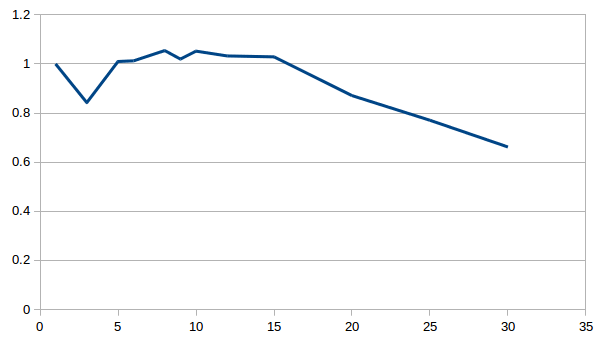
\includegraphics{eficiencia}

~\\
~\\
Realizaremos ademas otro tipo de mediciones. En este experimento se quiere dejar el tiempo limite en 120s, y medir cuanto trabajo pudo realizarse para distintas cantidades de unidades de procesamiento.
~\\
~\\ 
El programa fue nuevamente ejecutado en una red ethernet con 21 maquinas, cada una disponiendo de 3 núcleos. Al momento de realizar la experimentación, estas maquinas estaban siendo utilizadas, a razón de un núcleo por maquina, con lo cual se disponía de 63 núcleos para procesar la prueba. 
~\\
~\\
Se contó la cantidad de elementos del sistema calculados, que al fin y al cabo es lo que nos interesa calcular. Es importante aclarar que cuando en la tabla de resultados figura que se utilizó un solo núcleo, esa medición fue realizada sobre la versión serial del programa, no perdiendo así tiempo en inicializar las variables de MPI, calcular las secciones, y otras cuestiones que no son necesarias ne la versión serial. Por comodidad, la unidad de medida elegida para medir el trabajo fue millones de elementos calculados. Los resultados son los siguientes:
~\\
\begin{verbatim}
núcleos   trabajo
1         111.113
5         413.814
20        1976.24
35        3198.04
50        3661.31
60        4294.03
\end{verbatim}

Como podemos ver, estos se comportan linealmente, como puede verse en el siguiente gráfico:

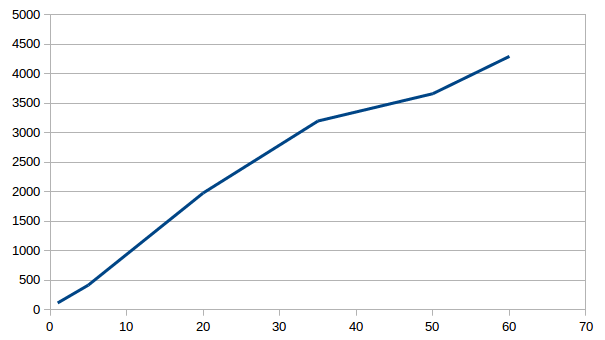
\includegraphics{Gustavson}

Si calculamos el trabajo realizado por cada núcleo obtenemos:
\begin{verbatim}
núcleos   trabajo/núcleos
1         111.113
5         82.7628
20        98.812
35        91.3725714286
50        73.2262
60        71.5671666667
\end{verbatim}

Y finalmente dividiendo este valor por el trabajo realizado por un núcleo, obtenemos una medida de cuanto trabajo logramos extraer por núcleo, al compararlo con una versión serial.
\newpage
\begin{verbatim}
núcleos   trabajo/(núcleos*111.113)
1         1
5         0.7448525375
20        0.889292882
35        0.8223391631
50        0.6590245966
60        0.6440935504
\end{verbatim}
El siguiente es el gráfico correspondiente a estos valores:

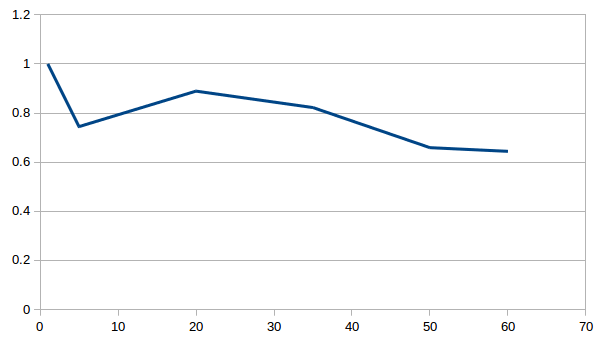
\includegraphics{Gustavson2}

 A primera vista parece que se pierde mucho rendimiento. En realidad, si tenemos en cuenta que la corrida de un solo nucleo fue realizada con una versio distinta que no incluye codigo de MPI, se entiende que ese valor aparezca como un outlier. Dicho esto, lo que esperariamos ver si el programa escalara, seria una recta horizontal. Si bien no es el resultado obtenido, no se dista mucho. Lo importante es que encontramos que se puede aumentar la cantidad de trabajo realizable significativamente agregando unidades de procesamiento, lo cual es un resultado mas optimista que el insinuado por la Ley de Amdahl.

\end{subsection}
\end{section}


\begin{section}{Conclusión}
Los resultados obtenidos sugieren que, como es sugerido por la Ley de Amdahl, intentar agregar unidades de procesamiento con la esperanza de reducir el tiempo de procesamiento que toma un trabajo dado es eficiente solo hasta cierto punto. La sección serial del programa pasará a dominar el tiempo de ejecución y no se podrá disminuir lo que toma en terminar.
~\\
~\\
Por otro lado, notamos que es beneficioso aumentar la carga de trabajo paralelo, ya que así el porcentaje de tiempo de procesador que se gasta en procesar datos aumenta cada vez mas, mientras que en comparación el tiempo utilizado en procesar la porción serial permanece pequeño. Esto nos indica que los tipos de procesamiento que se verán beneficiados del paralelismo son aquellos donde podamos incrementar fuertemente los cálculos realizados por la sección paralela, siendo las simulaciones realizadas mediante diferencias finitas un buen ejemplo de esto último.
\end{section}



\end{document}
